% verso e anverso:
% \documentclass[12pt,openright,twoside,a4paper,english]{abntex2}
% apenas verso:	
\documentclass[12pt,oneside,a4paper,english]{abntex2} 

\usepackage[alf]{abntex2cite}	% Citações padrão ABNT
\usepackage{listings}
\usepackage{float}
\usepackage{cmap}				% Mapear caracteres especiais no PDF
\usepackage{lmodern}			% Usa a fonte Latin Modern			
\usepackage[T1]{fontenc}		% Selecao de codigos de fonte.
\usepackage[utf8]{inputenc}		% Codificacao do documento (conversão automática dos acentos)
\usepackage{lastpage}			% Usado pela Ficha catalográfica
\usepackage{indentfirst}		% Indenta o primeiro parágrafo de cada seção.
\usepackage{color}				% Controle das cores
\usepackage{graphicx}			% Inclusão de gráficos
\usepackage{pdfpages}
\usepackage{tikz}
\usetikzlibrary{automata,positioning}
\usepackage{mathtools}

\definecolor{blue}{RGB}{41,5,195} % alterando o aspecto da cor azul

\makeatletter
\hypersetup{
    %pagebackref=true,
    pdftitle={\@title}, 
    pdfauthor={\@author},
    pdfsubject={\@title},
    pdfcreator={\imprimirpreambulo},
    pdfkeywords={Linguagens}{Compiladores}{Especificação do Ambiente de Execução}, 
    colorlinks=true,       		% false: boxed links; true: colored links
    linkcolor=blue,          	% color of internal links
    citecolor=blue,        		% color of links to bibliography
    filecolor=magenta,      		% color of file links
    urlcolor=blue,
    bookmarksdepth=4
}
\makeatother

\autor{Gustavo P. Gouveia (6482819), Victor Lassance (6431325)}
\title{Relatório de Compiladores\\Quarta Etapa\\Especificação do Ambiente de Execução\\Linguagem de programação \underline{CZAR}}
\orientador[Professor:]{Ricardo Luis de Azevedo da Rocha}
\preambulo{Texto apresentado à Escola Politécnica da Universidade de São Paulo como requisito para a aprovação na disciplina Linguagens e Compiladores no quinto módulo acadêmico do curso de graduação em Engenharia de Computação, junto ao Departamento de Engenharia de Computação e Sistemas Digitais (PCS).}
\instituicao{%
	Universidade de São Paulo
	\par
	Escola Politécnica
	\par
	Engenharia de Computação - Curso Cooperativo}
\local{São Paulo}
\data{2013}
\tipotrabalho{PCS2056 - Linguagens e Compiladores}

\setlength{\parindent}{1.3cm} % O tamanho do parágrafo
\setlength{\parskip}{0.2cm}  % Controle do espaçamento entre um parágrafo e outro

\makeindex

\begin{document}

\frenchspacing % Retira espaço extra obsoleto entre as frases.

\imprimirfolhaderosto

\tableofcontents

\textual

\chapter{Introdução}
\label{chap:introducao}
	% !TEX encoding = UTF-8 Unicode

Este projeto tem como objetivo a construção de um compilador de um só passo, dirigido por sintaxe, com analisador e reconhecedor sintático baseado em autômato de pilha estruturado.

Em um primeiro momento, foi definida uma linguagem de programação e identificados os tipos de átomos. Para cada átomo foi escrito uma gramática linear representativa da sua lei de formação e um reconhecedor para o átomo. Desse modo, as gramáticas assim escritas foram unidas e convertidas em um autômato finito, o qual foi transformado em um transdutor e implementado como sub-rotina, dando origem ao analisador léxico propriamente dito. Também foi criada uma função principal para chamar o analisador léxico e possibilitar o seu teste.

Durante a segunda etapa, a sintaxe da linguagem, denonimada por nós de CZAR, foi definida formalmente a partir de uma definição informal e de exemplos de programas que criamos, misturando palavras-chave e conceitos de diferentes linguagens de programação. As três principais definições foram escritas na notação BNF\footnote{Ver http://en.wikipedia.org/wiki/Backus\_Naur\_Form}, Wirth\footnote{Ver http://en.wikipedia.org/wiki/Wirth\_syntax\_notation} e com diagramas de sintaxe.

Na terceira etapa, implementamos o módulo referente à parte sintática para a nossa linguagem. O analisador sintático construído obtém uma cadeia de \emph{tokens} proveniente do analisador léxico, e verifica se a mesma pode ser gerada pela gramática da linguagem e, com isso, constrói a árvore sintática \cite{alfred1986compilers}.

Para a quarta entrega, focamos no ambiente de execução. O compilador por nós criado tem como linguagem de saída um programa que é executado na máquina virtual conhecida como Máquina de von Neumann (MVN).

Já durante as duas últimas entregas, complementamos a especificação do código gerado pelo compilador e das rotinas do ambiente de execução da nossa linguagem de alto nível, a CZAR. Além disso, buscamos integrar as rotinas semânticas no reconhecedor sintático de forma a permitir a geração de código e finalizar o compilador.

Como material de consulta, além de sites sobre o assunto e das aulas ministradas, foi utilizado o livro indicado pelo professor no começo das aulas \cite{intro-compiladores}, para pesquisa de conceitos e possíveis implementações.

O documento apresenta a seguir o processo completo de desenvolvimento de um compilador, desde a definição formal da linguagem, passando pelo analisador léxico, reconhecedor sintático, pela definição do ambiente de execução e das rotinas semânticas, terminando com um exemplo de programa traduzido.


\chapter{Instruções da Linguagem de Saída}
\label{chap:instrucoes-saida}
	% !TEX encoding = UTF-8 Unicode

TODO Listar e descrever instruções.


\chapter{Pseudoinstruções da Linguagem de Saída}
\label{chap:pseudoinstrucoes-saida}
	% !TEX encoding = UTF-8 Unicode

TODO Listar e descrever pseudoinstruções.


\chapter{Características Gerais}
\label{chap:caracteristicas-gerais}
	% !TEX encoding = UTF-8 Unicode

\section{Organização da memória}

O ambiente de execução da MVN fornece aos programadores um tamanho limitado de memória para ser usado no geral, a ser compartilhado entre o código e as variáveis do programa. O montador aloca a memória com base nos endereços relativos especificados no código do programa. Do total, a parte inicial da memória é reservada para guardar as instruções que serão executadas pelo programa. A parte final da memória deve ser usada especialmente para o uso do registro de ativação.

De maneira mais objetiva, reserva-se uma parte do código para a área de dados, uma parte para a função principal e as subrotinas e uma parte dedicada a pilhas de variáveis e endereços que viabilizam a chamada de subrotinas.

\section{Registro de ativação}

As funções em programas têm variáveis locais, que devem ser criadas na chamada da função e sobrevivem até que a função retorne. Elas também possuem recursão, onde cada instância da função tem seus próprios parâmetros e locais. As chamadas de funções se comportam de maneira LIFO, portanto podemos usar uma pilha como estrutura.

As operações push e pop dessa pilha não podem ser feitas individualmente para cada variável. Desa forma, manipula-se conjuntos de variáveis, e precisamos ter acesso a todas elas. Com isso, definimos dois conceitos:

\begin{itemize}
	\item \emph{Stack Pointer} (SP):
	\begin{itemize}
		\item Todas as posições além do SP são lixo;
		\item Todas as anteriores estão alocadas.
	\end{itemize}
	
	\item \emph{Activation Record} ou \emph{Stack Frame}
	\begin{itemize}
		\item área na pilha reservada para os dados de uma função (parâmetros, locais, endereço de retorno, etc).
	\end{itemize}
\end{itemize}

\begin{figure}[ht]
	\centering
	\caption{Esquema do Registro de Ativação}
	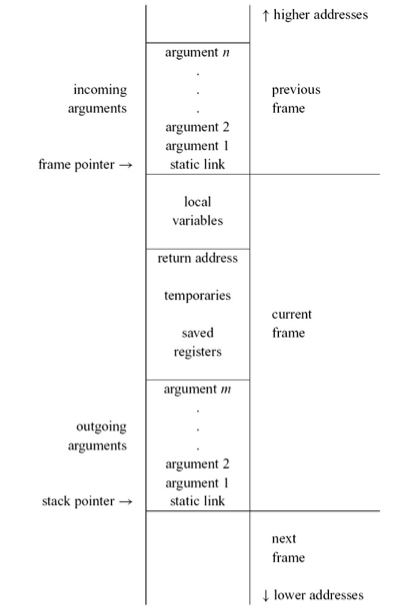
\includegraphics[width=0.5\textwidth]{images/registros-ativacao.png}
	\label{fig:registros-ativacao}
\end{figure}

A figura~\ref{fig:registros-ativacao} ilustra a organização da pilha. O uso do registro de ativação permite entre outras coisas a chamada recursiva de funções, uma vez isso não é possível de forma nativa no ambiente da MVN. No caso da MVN, a pilha cresce para baixo e as subrotinas são executadas utilizando as seguintes instruções:

\begin{itemize}
	\item Desvio para subprograma - mnemônico SC (0xA): armazena o endereço de instrução seguinte (atual + 1) na posição de memória apontada pelo operando. Em seguida, desvia a execução para o endereço indicado pelo operando e acrescido de uma unidade.
	
	\item Retorno de subprograma - mnemônico RS (0xB): desvia a execução para o endereço indicado pelo valor guardado na posição de memória do operando.
\end{itemize}

Foi criado por nós uma biblioteca em assembly para implementar funções auxiliares de entrada e saída de dados, além da funcionalidade de empilhar, desempilhar e ter acesso a informações contidas na pilha discutida anteriormente. Essas funções são explicadas na próxima seção.

	
\chapter{Biblioteca Desenvolvida em Assembly}
\label{chap:biblioteca-assembly}
	% !TEX encoding = UTF-8 Unicode

TODO Biblioteca Assembly

%\bibliography{bibliografia}

\end{document}
